\documentclass{standalone}
\usepackage{tikz}

\begin{document}
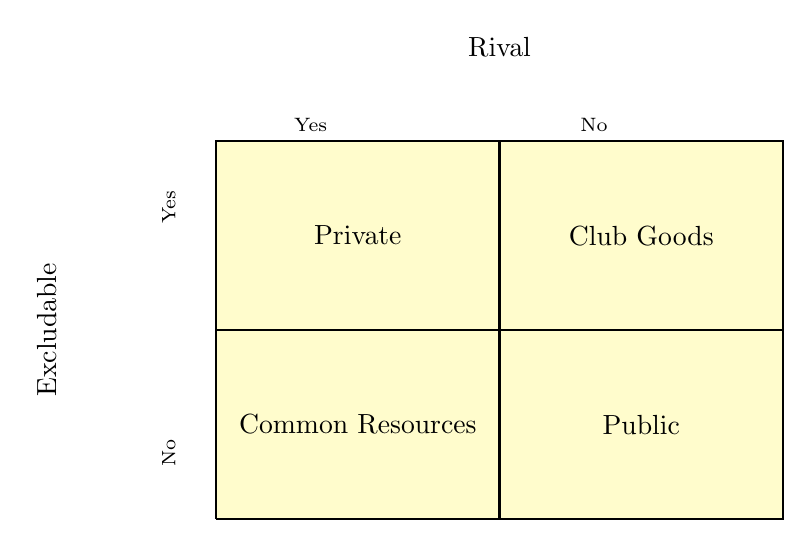
\begin{tikzpicture}[scale = 1.2]
%\draw[very thin, color = gray](0, 0) grid (12, 7);
\draw [thick, fill = yellow, fill opacity = 0.2] (3, 1) -- (6, 1) -- (6, 3) -- (3, 3) -- (3, 1);
%\draw [thick, fill = teal, fill opacity = 0.2] (6, 1) -- (6, 3) -- (3, 3);
\draw [thick, fill = yellow, fill opacity = 0.2] (6, 1) -- (9, 1) -- (9, 3) -- (6, 3) -- (6, 1);
%\draw [thick, fill = teal, fill opacity = 0.2] (9, 1) -- (9, 3) -- (6, 3);
\draw [thick, fill = yellow, fill opacity = 0.2] (6, 3) -- (9, 3) -- (9, 5) -- (6, 5) -- (6, 3);
%\draw [thick, fill = teal, fill opacity = 0.2] (9, 3) -- (9, 5) -- (6, 5);
\draw [thick, fill = yellow, fill opacity = 0.2] (3, 3) -- (6, 3) -- (6, 5) -- (3, 5) -- (3, 3);
%\draw [thick, fill = teal, fill opacity = 0.2] (6, 3) -- (6, 5) -- (3, 5);
\node at  (4.5, 2) {Common Resources};
\node at  (4.5, 4) {Private};
\node at  (7.5, 2) {Public};
\node at  (7.5, 4) {Club Goods};
%\node at  (6, 5) [below left] {1};
%\node at  (6, 1) [above right] {8};
%\node at  (9, 3) [below left] {8};
%\node at  (6, 3) [above right] {20};
%\node at  (9, 5) [below left] {0};
\node at (4, 5) [above] {\scriptsize Yes};
\node at (7, 5) [above] {\scriptsize No};
\node [rotate = 90] at (2.5, 1.7) {\scriptsize No};
\node [rotate = 90] at (2.5, 4.3) {\scriptsize Yes};
\node at (6, 6) {Rival};
\node [rotate = 90] at (1, 3) [below] {Excludable};
\end{tikzpicture}
\end{document}
